\documentclass[a4paper]{article}

\usepackage[portuguese]{babel} \usepackage[utf8]{inputenc}
\usepackage{indentfirst} \usepackage{graphicx} \usepackage{verbatim}
\usepackage[T1]{fontenc}
\usepackage{wrapfig}

\begin{document}

\setlength{\textwidth}{16cm} \setlength{\textheight}{22cm}

\title{\Huge\textbf{Protocolo de Ligação de
    Dados}\linebreak\linebreak\linebreak \Large\textbf{Relatório \\
    Trabalho1}\linebreak\linebreak 
\includegraphics[height=6cm,
    width=7cm]{feup.pdf}\linebreak \linebreak \Large{Mestrado Integrado em
    Engenharia Informática e Computação} \linebreak \linebreak \Large{Redes de
Computadores} }

\author{Hugo Ari Rodrigues Drumond --- 201102900 --- hugo.drumond@fe.up.pt \\
    José Pedro Pereira Amorim --- 201206111 --- ei12190@fe.up.pt \\ João
    Ricardo Pintas Soares --- 201200740 ---
    ei12039@fe.up.pt\linebreak\linebreak\linebreak \\ \\ Faculdade de
    Engenharia da Universidade do Porto \\ Rua Roberto Frias, 4200--65 Porto,
    Portugal \linebreak\linebreak\linebreak \linebreak\linebreak\vspace{1cm}}
    \maketitle \thispagestyle{empty}

\newpage

\section{Introdução}
%indicação dos objectivos do trabalho e do relatório; descrição da lógica do
%relatório com indicações sobre o tipo de informação que poderá ser encontrada
%em cada uma secções seguintes
Este trabalho laboratorial, desenvolvido no âmbito da Unidade Curricular de
Redes de Computadores (RCOM), teve como objetivo implementar um protocolo de
ligação de dados, do tipo acknowledged connection-oriented, e testá-lo em
diversas situações de stress de modo a verificar a sua robustez. Ao longo deste
relatório, serão descritos os aspetos fundamentais do referido trabalho,
permitindo obter um conhecimento detalhado deste. Será apresentada a
arquitetura, estrutura do código, casos de uso principais, protocolo de ligação
lógica e de aplicação. No mesmo sentido, serão apresentadas a validação dos
resultados e os elementos de valorização.

\section{Arquitectura}
%blocos funcionais e interfaces
O nosso software foi desenvolvido de maneira a tirar o máximo proveito da
estratégia de encapsulamento. O que permite: modificar, fazer novas
implementações, alterar técnicas de integridade de dados, etc, sem que haja
incompatibilidades ou quebra das interfaces de cada camada. Embora esta ideia de isolamento
tenha surgido nas linguagens de programação orientadas a objetos, o código em C
permite seguir este ideal pelo uso da palavra static. Tal, faz com que um
elemento só seja visível no ficheiro onde está declarado e definido. A técnica
usada pelo nosso código foi declarar a API (funções e estruturas de retorna de
informação public) de cada camada (classe) nos headers. E, nos respetivos ficheiros de código
fazer a definição da API\@; e a declaração e definição das funções e estruturas
auxiliares e de controlo com a palavra static (private).
\\\newline\textbf{Resultando no seguinte esboço arquitectural:}\\\newline
\centerline{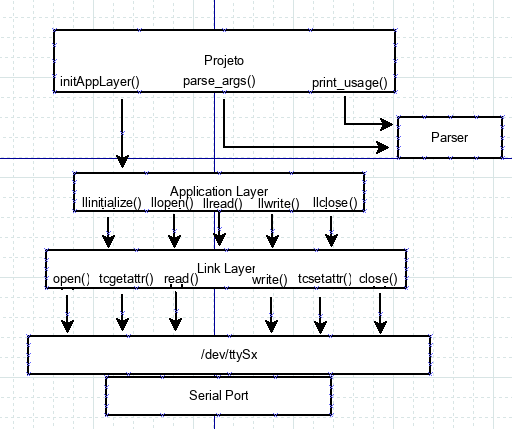
\includegraphics{API.png}}

\section{Estrutura do código}
%APIs, principais estruturas de dados, principais funções e sua relação com a
%arquitetura
\textbf{Estruturas:}\\
\begin{wrapfigure}{r}{0.3\textwidth}
  \begin{center}
    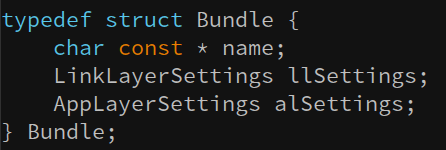
\includegraphics[width=0.45\textwidth]{bundleStruct.png}
    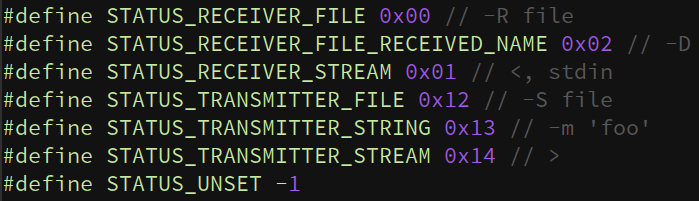
\includegraphics[width=0.45\textwidth]{status.png}
  \end{center}
\end{wrapfigure}
No \textit{bundle.h} encontra-se uma estrutura chamada Bundle cujo
objetivo é guardar os settings que recebemos da linha de comandos.
O name é um nome a que queremos chamar ao Bundle, e as estruturas
constituintes do Bundle são para os settings de cada camada. O
LinkLayerSettings está declarado no ficheiro linklayersettings.h e contem os
seguintes argumentos: port, timeout, numAttempts, payloadSize e baudrate.
O AppLayerSettings está declarado no ficheiro applayersettings.h e contem os
seguintes argumentos: status, packetBodySize, filename e um union Io que pode
ser um apontador para um ficheiro, para uma string ou nulo. Para alem disso,
encontram-se lá defines que o parser usa para indicar como aceder ao Union Io e
qual o modo de operação.\\\newline




\centerline{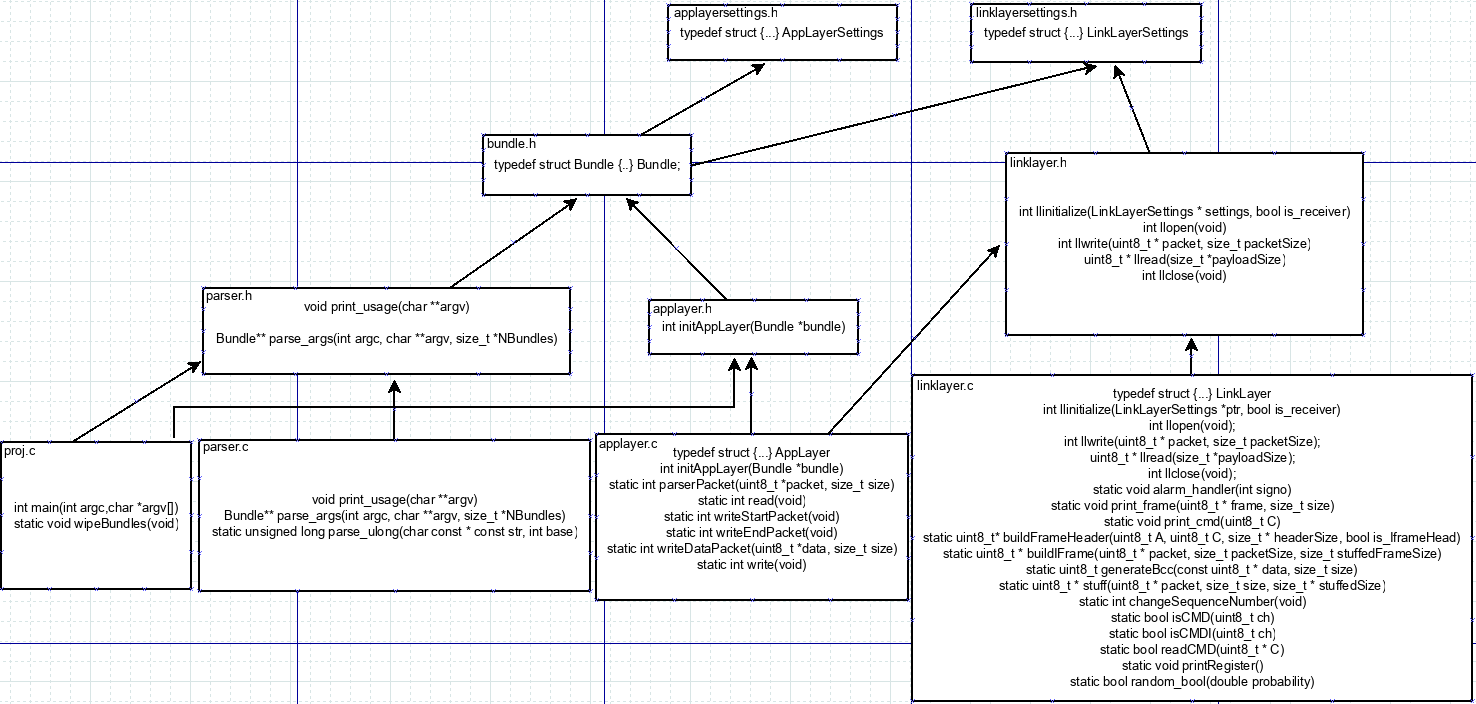
\includegraphics[scale=0.70]{organizacaoFicheirosECodigo.png}}


\section{Casos de uso}
%identificação; sequências de chamada de funções
O utilizador só pode interagir com a nossa aplicação através da linha de
comandos. Criámos um caso de usos bastante completo, que permite ao utilizador
mudar todas as opções do linkLayer e da applicacationLayer, que têm impacto na
transferência de dados. Para além disso, o parser aceita um número ilimitado de
portas séries quer sejam destinadas a receber ou enviar, e as respetivas
configurações. Cada uma separada com o símbolo +. Para ver quais as opções que
a nossa aplicação suporta basta corrê-la com a opção -h, serius -h. Também
incluímos alguns exemplos de uso. Lá podemos encontrar o nome Bundle que
basicamente significa um conjunto de opções (Options:) para uma dada porta
série que opera de uma dada maneira (Mode:), receptor ou emissor. Por
exemplo:\\\newline serius -d'/dev/tty100' -b115200 -t4 -r10 -f150 -s90
-S'pinguim.gif' + -d'/dev/tty200' -S'pinguim.gif'\\\newline Neste exemplo, os
seguintes settings são aplicados na porta série tty100: baudrate, timeout,
retries, tamanho máximo do payload (unstuffed) e o tamanho máximo da parte dos
dados do pacote de informação. E na tty200 os defaults são usados para todas
essas opções e para as restantes. Em ambos os casos as portas série atuam como
emissoras e enviam o ficheiro pinguim.gif para possivelmente computadores
diferentes. Um dos computadores receptores teria um processo serius iniciado
com os seguintes argumentos:\\\newline serius -d '/dev/tty300' -b 115200 -D\\
Cria um ficheiro com o nome que vem no pacote de controlo start, e coloca lá a
informação que recebe. \\\newline E o outro:\\\newline serius -d '/dev/tty400'
-R 'received.gif' \\\newline De início, tínhamos em mente correr cada Bundle
numa thread. Possibilitando transferir/receber de várias fontes simultâneamente
via porta série, no entanto, não houve tempo para o fazer. O mesmo sucedeu com
as pipes e a redireção da shell, cuja ideia era respetivamente: enviar
informação acabada de ser processada; e, método alternativo de guardar
ficheiros ou de os receber.\\Entre a opção e o argumento tanto faz haver
ou nao haver espaços, -b115200 = -b 115200.
\\\newline\textbf{Diagrama de casos de uso:}\\\newline
\centerline{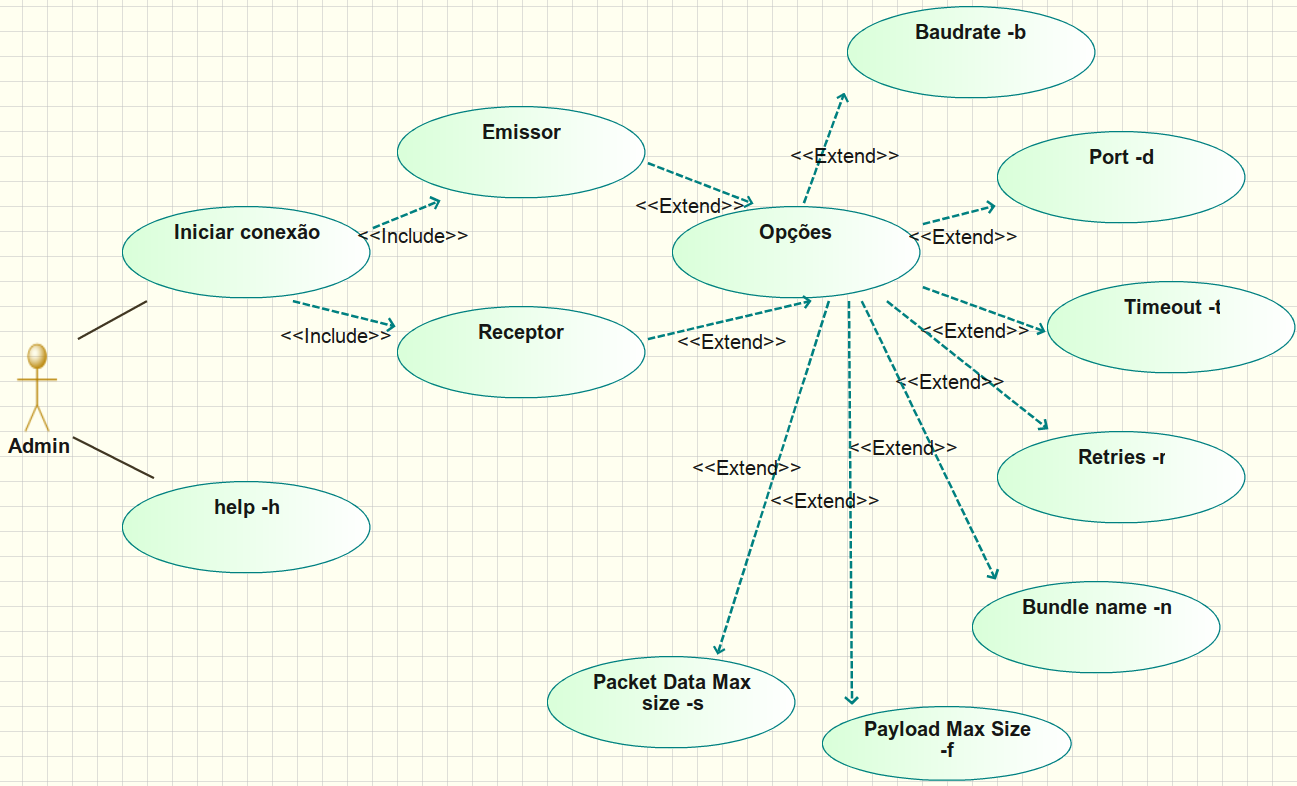
\includegraphics[scale=0.6]{useCases.png}}

\section{Protocolo de ligação lógica}
%identificação dos principais aspectos funcionais; descrição da estratégia de
%implementação destes aspectos com apresentação de extratos de código

\section{Protocolo de aplicação}
%identificação dos principais aspectos funcionais; descrição da estratégia de
%implementação destes aspectos com apresentação de extractos de código

\section{Validação}
%descrição dos testes efectuados com apresentação quantificada dos resultados,
%se possível

\section{Elementos de valorização}
%identificação dos elementos de valorização implementados; descrição da
%estratégia de implementação com apresentação de pequenos extratos de código

\section{Conclusões}
%síntese da informação apresentada nas secções anteriores; reflexão sobre os
%objectivos de aprendizagem alcançados

\end{document}
